\documentclass[11pt]{article}

% open-provenance: An Open, Offline, User-Governed System for Verifiable Media Provenance
% Draft technical report. Compile: see docs/paper/README.md.

\usepackage[utf8]{inputenc}
\usepackage[margin=1in]{geometry}
\usepackage{amsmath,amssymb}
\usepackage{booktabs}
\usepackage{graphicx}
\usepackage{enumitem}
\usepackage[numbers,sort&compress]{natbib}
\usepackage[hidelinks]{hyperref}

\newcommand{\state}[1]{\textsc{#1}}

\title{\textbf{open-provenance}: An Open, Offline, User-Governed System\\
for Verifiable Media Provenance and Durable Recovery}
\author{Abu Sufian Sarkar\\\texttt{abu@cyberdude.com}}
\date{\today}

\begin{document}
\maketitle

\begin{abstract}
The marginal cost of producing convincing synthetic images, audio, and video has fallen to
near zero, eroding society's shared ability to answer a basic question: \emph{did this
actually happen?} We argue that the tractable response is not universal \emph{detection} of
synthetic media---which the literature shows to be brittle and adversarially
fragile---but verifiable \emph{provenance}: cryptographically signed, content-bound
statements about how a piece of media came to be. We present \textbf{open-provenance}, an
open-source system built on the C2PA standard that makes provenance verification (i)
\emph{offline}, requiring no network and no trusted third party at verification time; (ii)
\emph{user-governed}, so that the decision of \emph{whom to trust} rests with the verifier
rather than a central gatekeeper; and (iii) \emph{honest}, with a conservative verdict
model that never conflates an intact provenance chain with the truth of the depicted
events, and never treats the absence of provenance as evidence of fabrication. We further
study the central weakness of metadata-based provenance---that it is stripped by
screenshots and social-media re-encoding---and prototype a \emph{durable} recovery layer
combining a perceptual-fingerprint registry with robust watermarking. On the Kodak
natural-image suite, fingerprint-based recovery is robust to recompression and rescaling
(ROC AUC $=1.0$; mean Hamming distance $0.22$ vs.\ $23.11$ of $64$ between matching and
non-matching content under resize-to-$70\%$ + JPEG-$40$ transport), but \emph{degrades
under cropping}---nearest-neighbour recovery falls from $1.0$ to $0.50$ as the retained
area shrinks to $70\%$---while a lightweight frequency-domain watermark fails by JPEG
quality $\approx 50$. These results delimit, rather than oversell, what the open layer
achieves, and motivate crop-robust learned watermarks. We are explicit about scope: the
open ecosystem cannot read proprietary watermarks (e.g.\ SynthID), so durable recovery
protects content that passes through participating signers, not arbitrary third-party
media. All code, the evaluation harness, and this report are released openly.
\end{abstract}

\section{Introduction}
Generative models now synthesize photorealistic media indistinguishable from captured
reality~\cite{rombach2022ldm}. This is not a niche concern: the ability to attribute media
to a source underpins journalism, legal evidence, scientific record, elections, and
ordinary interpersonal trust. Two broad technical responses exist. \emph{Detection} asks a
classifier whether a given artifact is synthetic; it is a moving target, content- and
model-specific, and degrades under distribution shift and adversarial
post-processing~\cite{verdoliva2020media,farid2016photo}. \emph{Provenance} instead attaches
verifiable, signed statements to media at creation and edit time, shifting the question from
``does this look fake?'' to ``what is this artifact's documented history, and do I trust the
party that attests to it?''

We take the provenance position, and observe that a provenance system intended as shared
infrastructure must satisfy three properties that existing deployments only partially meet.
First, \textbf{verification must be a public good}: it should require no account, no
gatekeeper, and---critically---no network, so that a journalist in the field or a court
clerk can verify locally. Second, \textbf{trust must be user-governed}: a verifier that
ships a fixed list of ``legitimate'' signers is itself a central arbiter of authenticity,
which is precisely the concentration of power a neutral system should avoid. Third, the
system must be \textbf{epistemically honest}: it must distinguish ``the cryptographic chain
is intact'' from ``the depicted events are true,'' and must never present the mere absence
of provenance as evidence of manipulation.

\paragraph{Contributions.}
\begin{enumerate}[noitemsep]
\item An open verifier with a conservative, formally specified verdict and trust model that
encodes the honesty properties above (\S\ref{sec:design}), realized as both an offline CLI
and a zero-backend in-browser WebAssembly application.
\item A user-governed trust mechanism in which the verifier cryptographically validates the
signer's certificate chain against anchors the \emph{user} supplies, with no built-in
default trust list (\S\ref{sec:design}).
\item A study and open prototype of \emph{durable} provenance recovery---surviving metadata
stripping---combining a perceptual-fingerprint registry with robust watermarking, with a
reproducible evaluation (\S\ref{sec:eval}).
\item An explicit threat model and an honest account of what open provenance can and cannot
do, including the proprietary-watermark gap (\S\ref{sec:threat},~\S\ref{sec:discussion}).
\end{enumerate}

\section{Background and Related Work}
\paragraph{Provenance standards.} The C2PA specification~\cite{c2pa-spec} defines a
\emph{manifest}: a set of assertions about an asset (capture device, edits, ingredients)
bound to the asset's pixels by cryptographic hashes, and signed using a COSE
structure~\cite{rfc9052} whose signer is identified by an X.509 certificate
chain~\cite{rfc5280}, optionally timestamped via RFC~3161~\cite{rfc3161}. The Content
Authenticity Initiative~\cite{cai} promotes adoption (``Content Credentials''). The IPTC
\texttt{digitalSourceType} vocabulary~\cite{iptc-dst} provides the standard marker for
algorithmically generated media (\texttt{trainedAlgorithmicMedia}).

\paragraph{Watermarking.} Classical invisible watermarking embeds a payload in transform
coefficients (DWT/DCT/SVD)~\cite{cox2008watermarking,invisiblewatermark}; such methods
survive mild recompression and scaling but are fragile under strong compression and
geometric distortion. Learned watermarks embed and detect payloads with neural networks and
are markedly more robust: Stable Signature roots a watermark in a diffusion model's
decoder~\cite{fernandez2023stable}; TrustMark targets arbitrary-resolution robustness for
C2PA soft binding~\cite{bui2023trustmark}; WAM localizes messages and resists
cropping~\cite{sander2024wam}; SynthID is a widely deployed but proprietary
scheme~\cite{synthid,dathathri2024synthid}.

\paragraph{Fingerprinting.} Perceptual hashes summarize low-frequency image structure into
compact codes stable under recompression and scaling~\cite{zauner2010phash}, enabling
content matching against a registry. The combination of robust watermark, fingerprint, and
manifest registry is the basis of ``durable'' Content Credentials~\cite{durable-cc}.

\section{Threat Model}\label{sec:threat}
\paragraph{Goals.} For a verifier $V$ presented with an asset $a$, the system should provide
(G1)~\emph{integrity}---detect any modification of $a$ after signing; (G2)~\emph{authenticity
of the signer}---establish, relative to $V$'s chosen trust anchors, which party signed $a$;
(G3)~\emph{recoverability}---when $a$'s manifest has been stripped, recover it for content
previously registered by a participating signer.

\paragraph{Adversary.} We consider an adversary who may: strip or alter manifest metadata;
recompress and rescale (lossy transport via screenshots and social platforms); crop or
geometrically distort; substitute or self-sign with an attacker-controlled certificate
(forge signer identity); and replay a valid manifest onto different content. The adversary
does \emph{not} possess the private keys of signers $V$ trusts, and cannot break the
underlying signature or hash primitives.

\paragraph{Non-goals.} The system does \emph{not} establish that the events depicted in $a$
are true (a correctly signed photograph may still be staged), does \emph{not} detect
unmarked synthetic media, and does \emph{not} read third-party proprietary watermarks. The
absence of provenance is treated as \emph{uninformative}, never as evidence of fabrication.

\section{System Design}\label{sec:design}
\subsection{Honest verdict model}
Given the validation outcome of a C2PA read, the verifier emits exactly one verdict
$\in \{\state{verified}, \state{no\_credentials}, \state{invalid}\}$:
\begin{itemize}[noitemsep]
\item \state{verified}: a manifest is present and all signature and content-hash checks
pass. This asserts chain integrity only.
\item \state{no\_credentials}: no manifest is present. Formally uninformative about
authenticity.
\item \state{invalid}: a manifest is present but a hash or signature check fails; the asset
was altered after signing or the chain is broken.
\end{itemize}
Orthogonally, the verifier reports a trust status
$\in \{\state{trusted}, \state{untrusted}, \state{unchecked}\}$. Let $C$ be the signer's
certificate chain and $\mathcal{A}$ the user's set of trust anchors. Then
\[
\text{trust}(C,\mathcal{A}) =
\begin{cases}
\state{trusted} & \text{if } C \text{ chains to some anchor in } \mathcal{A},\\
\state{untrusted} & \text{if } \mathcal{A}\neq\emptyset \text{ and } C \text{ does not},\\
\state{unchecked} & \text{if } \mathcal{A}=\emptyset \text{ (or no trust engine)}.
\end{cases}
\]
Crucially, \state{verified} is independent of trust: a cryptographically valid signature
from an untrusted (e.g.\ self-signed) party yields $\langle\state{verified},
\state{untrusted}\rangle$, which the interface presents as a warning, never as an
endorsement.

\subsection{Offline verification and user-governed trust}
Because the signer's certificate travels inside the manifest, verification is
\emph{permissionless} and \emph{local}: no network is contacted. The in-browser implementation
disables remote-manifest fetching and OCSP, guaranteeing that no request leaves the device.
Trust is supplied by the user as a set of PEM anchors; the toolkit validates $C$ against
$\mathcal{A}$ on-device. The system ships \emph{no} default trust list, by design: adopting
a published list (e.g.\ the C2PA list) is the user's explicit choice, not an imposed policy.

\subsection{Durable recovery layer}
Metadata-based provenance is fragile: most platforms strip C2PA manifests. We therefore
register, at signing time, a mapping from a robust descriptor of the content to its
manifest. Two descriptors are used. A \emph{perceptual fingerprint} $\phi(a)\in\{0,1\}^{64}$
(a DCT perceptual hash) supports registry lookup by nearest Hamming distance; recovery
declares a match iff $\min_e \mathrm{Ham}(\phi(a'), \phi_e) \le \tau$ for a threshold $\tau$,
framing recovery as a detection problem with an ROC over $\tau$. An optional \emph{robust
watermark} embeds a short identifier directly in pixels, giving a self-contained pointer that
needs no registry. The recovered manifest is then re-verified by the normal offline path.

\section{Implementation}
The verifier is implemented twice over a single shared, dependency-free verdict classifier:
a Node.js CLI using \texttt{c2pa-node}, and a zero-backend browser application that compiles
the C2PA toolkit to WebAssembly so verification runs client-side and offline. A signing tool
emits manifests (optionally tagging generative content via \texttt{digitalSourceType}). The
durable layer is implemented in Python over a DWT-DCT-SVD watermark~\cite{invisiblewatermark}
and a DCT perceptual hash~\cite{zauner2010phash}, with a registry supporting
\texttt{register} and \texttt{recover}. The evaluation harness (\S\ref{sec:eval}) regenerates
every quantitative claim in this report from a single command.

\section{Evaluation}\label{sec:eval}
\paragraph{Methodology.} We evaluate on the Kodak natural-image suite~\cite{kodak} ($18$ true-colour
$512\times768$ photographs with rich texture). A controlled synthetic corpus (sums of
low-frequency sinusoids) served as a sanity baseline during development and gave conclusions
consistent with those below for recompression and scaling; because smooth synthetic content
is favourable to perceptual hashing, we report only the natural-image results here. Realistic
transport includes JPEG recompression, rescaling, and---critically---\emph{center cropping},
the geometric distortion that frequency-domain watermarks and perceptual hashes are least
robust to. All results are produced by \texttt{eval/natural\_eval.py} and are fully
reproducible (corpus via \texttt{eval/fetch\_corpus.sh}).

\paragraph{N1: watermark robustness.} We embed a $64$-bit identifier and measure bit-error
rate (BER) and exact-recovery rate after JPEG recompression and rescaling
(Table~\ref{tab:n1}). On natural images the lightweight DWT-DCT-SVD watermark is reliable
only at high quality (exact recovery $1.0$ at $q\!=\!90$), degrades sharply by $q\!=\!70$
(exact recovery $0.33$), and is effectively destroyed by $q\!=\!50$ (BER $\ge 0.16$). It is
\emph{more} fragile on natural images than on smooth content, confirming that lightweight
frequency-domain watermarking is unsuitable for social-media-grade compression and
motivating learned schemes~\cite{bui2023trustmark,sander2024wam} for the embedded path.

\begin{table}[t]
\centering
\caption{N1 (Kodak): watermark bit-error rate and exact-recovery rate vs.\ JPEG quality and
rescale factor ($18$ images per condition).}
\label{tab:n1}
\begin{tabular}{rrrr}
\toprule
JPEG $q$ & scale & mean BER & exact-rec. \\
\midrule
90 & 1.00 & 0.000 & 1.00 \\
90 & 0.70 & 0.009 & 0.75 \\
70 & 1.00 & 0.043 & 0.29 \\
70 & 0.70 & 0.058 & 0.25 \\
50 & 1.00 & 0.176 & 0.00 \\
50 & 0.70 & 0.239 & 0.00 \\
30 & 1.00 & 0.435 & 0.00 \\
30 & 0.70 & 0.443 & 0.00 \\
\bottomrule
\end{tabular}

\end{table}

\paragraph{N2: durable recovery under recompression and scaling.} Using a leave-one-out
protocol, each registered image is transported (resize-to-$70\%$ + JPEG-$40$) and matched
against the gallery; \emph{mated} distances are to the correct entry and \emph{impostor}
distances to the nearest wrong entry. Matching content sits at mean Hamming distance
$0.22/64$ versus $23.11/64$ for non-matching content---a wide separation yielding the ROC in
Figure~\ref{fig:natroc} (AUC $=1.0$; equal-error rate at threshold $2$, recovery $1.0$ at
false-match $0.0$). Recovery thus succeeds on \emph{natural} images after transport that
destroys the watermark, establishing the fingerprint registry as the robust primary path for
this transport class.

\begin{figure}[t]
\centering
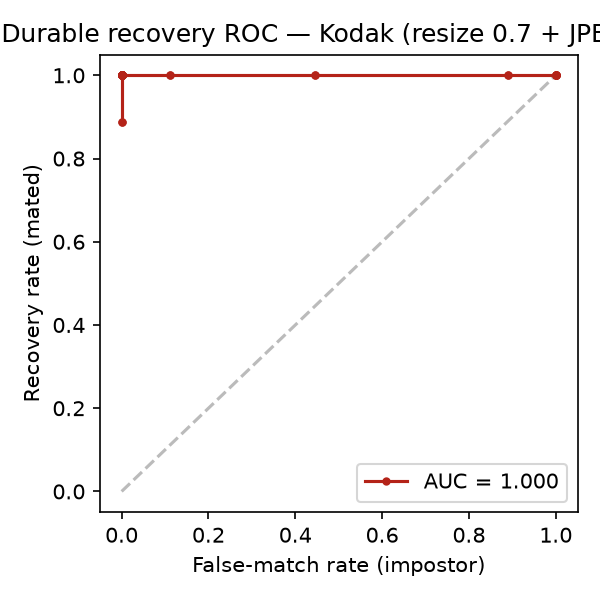
\includegraphics[width=0.5\linewidth]{figures/nat_roc.png}
\caption{N2 (Kodak): ROC for fingerprint-based recovery (mated vs.\ impostor, leave-one-out)
under resize-$0.7$ + JPEG-$40$ transport.}
\label{fig:natroc}
\end{figure}

\paragraph{N3: crop sensitivity (the honest stress test).} Perceptual hashing is not
translation- or crop-invariant, so we measure nearest-neighbour recovery as a function of the
retained center fraction (Table~\ref{tab:n3}). Recovery is perfect when at least $90\%$ of
the image is retained, but falls to $0.83$ at a $20\%$ crop and to $0.50$ at a $30\%$ crop, as
the mean mated distance grows from $0.4$ to $25.6/64$. Cropping is therefore the principal
failure mode of the fingerprint path---a limitation it shares with the DWT watermark---and
the strongest argument for crop-robust localized watermarks~\cite{sander2024wam} and
region/keypoint-based fingerprints in future work. We report this prominently rather than
averaging it away.

\begin{table}[t]
\centering
\caption{N3 (Kodak): nearest-neighbour recovery rate and mean mated Hamming distance vs.\
retained center-crop fraction (each crop followed by JPEG-$70$).}
\label{tab:n3}
\begin{tabular}{rrr}
\toprule
crop (keep) & recovery rate & mean mated dist. \\
\midrule
1.00 & 1.00 & 0.4 \\
0.95 & 1.00 & 4.3 \\
0.90 & 1.00 & 8.8 \\
0.80 & 0.83 & 18.8 \\
0.70 & 0.50 & 25.6 \\
\bottomrule
\end{tabular}

\end{table}

\section{Discussion}\label{sec:discussion}
The asymmetry of provenance is its defining property: \emph{signing is opt-in, verification
is universal}. Only content a creator chose to sign carries credentials, but anyone may
verify it without permission. This makes ``no credentials'' the common case in the wild and
is why honest messaging matters. Our results also delineate the open ecosystem's boundary.
Robust pixel watermarks deployed by major generative services (e.g.\ SynthID) are detectable
\emph{only} with proprietary, key-gated detectors; the open system cannot recover a stripped
third-party asset's provenance. Durable recovery here therefore protects content that passes
through \emph{participating} signers---a meaningful but bounded guarantee, and an argument for
open, interoperable robust-watermarking standards.

\section{Limitations and Ethics}
The evaluation uses $18$ natural images at modest scale; larger and adversarial benchmarks
(diverse sources, learned-attack post-processing) remain future work. The principal
technical limitation is geometric: recovery degrades sharply under cropping
(Table~\ref{tab:n3}), so the present fingerprint path should not be relied on against an
adversary who crops or warps. The fingerprint path also requires prior registration and is a
fuzzy match; at scale it needs collision handling and a registry whose governance is itself a
non-gatekeeping design problem. Offline revocation is unhandled: a revoked-but-still-chaining
certificate currently reads as trusted. Ethically, the system is designed against two failure modes: over-trust
(presenting an untrusted or merely-valid signature as endorsement) and the ``liar's
dividend'' (treating missing provenance as proof of fakery); both are explicitly precluded by
the verdict model. Registries of fingerprints carry privacy implications that a deployment
must address.

\section{Reproducibility}
All artifacts---verifier, signer, durable registry, and the evaluation harness that produced
Tables~\ref{tab:n1}--\ref{tab:n3} and Figure~\ref{fig:natroc}---are released under the
Apache-2.0 license. The natural-image numbers are regenerated by \texttt{eval/fetch\_corpus.sh}
followed by \texttt{python3 eval/natural\_eval.py}; library versions are pinned in the
repository.

\section{Future Work}\label{sec:future}
Crop robustness is the priority: localized learned watermarks~\cite{sander2024wam} and
region/keypoint-based fingerprints to withstand the cropping that defeats the present pHash
(Table~\ref{tab:n3}). Beyond that: larger and adversarial natural-image and video benchmarks;
integration of a learned watermark~\cite{bui2023trustmark} for compression-robust embedded
identifiers; offline revocation and trust-list distribution without a central authority; a
decentralized, privacy-preserving recovery registry; and standardization of an open
robust-watermark soft binding to close the third-party gap.

\bibliographystyle{plainnat}
\bibliography{references}

\end{document}
